\documentclass[man]{apa6}
\usepackage{lmodern}
\usepackage{amssymb,amsmath}
\usepackage{ifxetex,ifluatex}
\usepackage{fixltx2e} % provides \textsubscript
\ifnum 0\ifxetex 1\fi\ifluatex 1\fi=0 % if pdftex
  \usepackage[T1]{fontenc}
  \usepackage[utf8]{inputenc}
\else % if luatex or xelatex
  \ifxetex
    \usepackage{mathspec}
  \else
    \usepackage{fontspec}
  \fi
  \defaultfontfeatures{Ligatures=TeX,Scale=MatchLowercase}
\fi
% use upquote if available, for straight quotes in verbatim environments
\IfFileExists{upquote.sty}{\usepackage{upquote}}{}
% use microtype if available
\IfFileExists{microtype.sty}{%
\usepackage{microtype}
\UseMicrotypeSet[protrusion]{basicmath} % disable protrusion for tt fonts
}{}
\usepackage{hyperref}
\hypersetup{unicode=true,
            pdftitle={Personality and political beliefs across the lifespan},
            pdfauthor={Sarah Dimakis, Meghan Siritzky, \& Jamie Yellowtail},
            pdfkeywords={keywords: personality, openness to experiences, conscientiousness,
extraversion, agreeableness, emotional stability, conservatism, social
conservatism, economic conservatism},
            pdfborder={0 0 0},
            breaklinks=true}
\urlstyle{same}  % don't use monospace font for urls
\usepackage{graphicx,grffile}
\makeatletter
\def\maxwidth{\ifdim\Gin@nat@width>\linewidth\linewidth\else\Gin@nat@width\fi}
\def\maxheight{\ifdim\Gin@nat@height>\textheight\textheight\else\Gin@nat@height\fi}
\makeatother
% Scale images if necessary, so that they will not overflow the page
% margins by default, and it is still possible to overwrite the defaults
% using explicit options in \includegraphics[width, height, ...]{}
\setkeys{Gin}{width=\maxwidth,height=\maxheight,keepaspectratio}
\IfFileExists{parskip.sty}{%
\usepackage{parskip}
}{% else
\setlength{\parindent}{0pt}
\setlength{\parskip}{6pt plus 2pt minus 1pt}
}
\setlength{\emergencystretch}{3em}  % prevent overfull lines
\providecommand{\tightlist}{%
  \setlength{\itemsep}{0pt}\setlength{\parskip}{0pt}}
\setcounter{secnumdepth}{0}
% Redefines (sub)paragraphs to behave more like sections
\ifx\paragraph\undefined\else
\let\oldparagraph\paragraph
\renewcommand{\paragraph}[1]{\oldparagraph{#1}\mbox{}}
\fi
\ifx\subparagraph\undefined\else
\let\oldsubparagraph\subparagraph
\renewcommand{\subparagraph}[1]{\oldsubparagraph{#1}\mbox{}}
\fi

%%% Use protect on footnotes to avoid problems with footnotes in titles
\let\rmarkdownfootnote\footnote%
\def\footnote{\protect\rmarkdownfootnote}


  \title{Personality and political beliefs across the lifespan}
    \author{Sarah Dimakis\textsuperscript{1}, Meghan Siritzky\textsuperscript{1}, \&
Jamie Yellowtail\textsuperscript{1}}
    \date{}
  
\shorttitle{PERSONALITY AND POLITICAL BELIEFS}
\affiliation{
\vspace{0.5cm}
\textsuperscript{1} University of Oregon}
\keywords{keywords: personality, openness to experiences, conscientiousness, extraversion, agreeableness, emotional stability, conservatism, social conservatism, economic conservatism\newline\indent Word count: 208}
\usepackage{csquotes}
\usepackage{upgreek}
\captionsetup{font=singlespacing,justification=justified}

\usepackage{longtable}
\usepackage{lscape}
\usepackage{multirow}
\usepackage{tabularx}
\usepackage[flushleft]{threeparttable}
\usepackage{threeparttablex}

\newenvironment{lltable}{\begin{landscape}\begin{center}\begin{ThreePartTable}}{\end{ThreePartTable}\end{center}\end{landscape}}

\makeatletter
\newcommand\LastLTentrywidth{1em}
\newlength\longtablewidth
\setlength{\longtablewidth}{1in}
\newcommand{\getlongtablewidth}{\begingroup \ifcsname LT@\roman{LT@tables}\endcsname \global\longtablewidth=0pt \renewcommand{\LT@entry}[2]{\global\advance\longtablewidth by ##2\relax\gdef\LastLTentrywidth{##2}}\@nameuse{LT@\roman{LT@tables}} \fi \endgroup}


\DeclareDelayedFloatFlavor{ThreePartTable}{table}
\DeclareDelayedFloatFlavor{lltable}{table}
\DeclareDelayedFloatFlavor*{longtable}{table}
\makeatletter
\renewcommand{\efloat@iwrite}[1]{\immediate\expandafter\protected@write\csname efloat@post#1\endcsname{}}
\makeatother

\authornote{This project was completed as part of the EDLD
Introduction to Data Science class at the University of Oregon.

Correspondence concerning this article should be addressed to Sarah
Dimakis, University of Oregon, Eugene, OR. E-mail:
\href{mailto:sdimakis@uoregon.edu}{\nolinkurl{sdimakis@uoregon.edu}}}

\abstract{
Since the development of the Five Factor Model as a framework for
measuring and classifying personality, psychology research has been
interested in using this framework to examine the relationship between
personality and cognitions, mindsets, and behaviors. Prior research has
attempted to predict political beliefs and affiliations from personality
traits, finding that the personality trait of openness to experience is
positively correlated with liberalness, while the trait of
conscientiousness is positively correlated with conservativeness. The
current study attempts to replicate these findings in a U.S. Amazon
Mechanical Turk population using the Ten Item Personality Inventory to
measure the Big Five personality traits (openness to experiences,
conscientiousness, extraversion, agreeableness, and emotional stability)
and a 12-item Social and Economic Conservatism Scale to measure the
social and economic dimensions of conservatism. Consistent with past
research, the current study found that openness to experience was a
significant negative predictor of both economic and social conservatism.
Contrary to past findings, however, we found that agreeableness and
emotional stability were both significant positive predictors of social
conservatism, and conscientiousness was not a significant predictor of
either social or economic conservatism. Neither social nor economic
conservatism were strongly correlated with any of the Big Five
personality traits, but they were strongly positively correlated with
each other.


}

\begin{document}
\maketitle

The Five Factor Model is a widely used framework for measuring and
classifying personality into five dimensions (Goldberg, 1992; John \&
Srivastava, 1999; McCrae et al., 1999). Those who score high in
\emph{openness to experiences} tend to describe themselves as curious,
deep thinkers compared to those who score low in openness to experience,
who describe themselves as traditional and conventional. Those who score
high in \emph{conscientiousness} are generally reliable and hardworking,
while those who score low in conscientiousness tend to be disorganized
and impulsive. Those high in \emph{extraversion} are talkative and
energetic, while those high in introversion are reserved and quiet.
Those who score high in \emph{agreeableness} describe themselves as kind
and trusting, while those who score low in agreeableness say they are
quarrelsome and critical. And lastly, those who are high in
\emph{emotional stability} are calm individuals who handle stress well,
while those high in neuroticism tend to be anxious individuals who are
easily upset.

Given that these personality traits have been found to predict a
multitude of cognitions and behaviors, from well-being to cognitive
abilities (Barlett \& Anderson, 2012; Curtis, Windsor, \& Soubelet,
2015; Hayes \& Joseph, 2003), previous studies have looked at whether
personality can predict political beliefs and affiliation (Hirsh,
DeYoung, Xu, \& Peterson, 2010; Jost, West, \& Gosling, 2009). The most
robust findings are that openness to experience is positively correlated
with liberalness (Carney, Jost, Gosling, \& Potter, 2008; Ekehammar,
Akrami, Gylje, \& Zakrisson, 2004), while conscientiousness is
positively correlated with conservativeness (Barbaranelli, Caprara,
Vecchione, \& Fraley, 2007; Stenner, 2005).

This project uses data from a larger study that measured political
beliefs and the big five personality traits. Consistent with prior
research, we hypothesize that we will find a positive relation between
conscientiousness and conservatism and a negative relation between
openness to experience and conservatism. We will first make exploratory
tables and plots that explore the relation between all big five
personality traits and social and economic conservatism, and then we
will run two linear models with traits as predictors and types of
conservatism as outcome variables.

\section{Method}\label{method}

\subsection{Participants}\label{participants}

Two-hundred U.S. adults were recruited via Amazon Mechanical Turk to
participate in a study listed as \enquote{Psychology and society
survey.} Participants were removed for completing the survey quicker
than predetermined time cutoffs or failing to pass attention checks. Of
the remaining 131 participants, who were 20 to 68 years old (\emph{M} =
40.55, \emph{SD} = 11.98), 54.2\% identified as female and 45.8\%
identified as male, while 77.1\% identified as White of Caucasian, 7.6\%
as African American or Black, 6.1\% as Hispanic or Latinx, 5.3\% as
Asian or Asian American, 0.8\% as Native American, and 9.2\% as
\enquote{Other.} The sample leaned liberal, with 45\% affiliated with
the Democratic Party, 23.7\% affiliated with the Republican Party,
22.1\% affiliated with no party, and 9.2\% affiliated with the Green
Party, Libertarian Party, or another party. The participants were
compensated \$1.50 for completing the survey, which took on average
10.43 minutes (\emph{SD} = 3.34).

\subsection{Material}\label{material}

\textbf{Personality.} To assess personality traits (openness to
experiences, conscientiousness, extraversion, agreeableness, and
emotional stability), respondents completed the Ten Item Personality
Inventory (Gosling, Rentfrow, \& Swann Jr, 2003). Participants were
asked to indicate the extent to which they agreed or disagreed with
statements describing themselves (e.g. \enquote{Extraverted,
enthusiastic}; \enquote{Critical, quarrelsome}). Respondents rated each
statement on a 7-point likert scale (1 = Strongly Disagree to 7 =
Strongly Agree). Responses were coded such that higher values reflected
greater identification with the personality trait.

\textbf{Social and Economic Conservatism.} To assess participant levels
of conservatism, respondents completed the 12-item Social and Economic
Conservatism Scale (Everett, 2013). Participants were asked to indicate
the extent to which they feel positively or negatively about seven
social issues and five economic issues (eg. Abortion; Fiscal
Responsibility). Respondents rated each issue on a 100-point scale (0
indicates greater negativity and 100 indicates greater positivity).
Responses were coded such that higher values reflected greater levels of
conservatism.

\textbf{Additional Measures.} Incidental affect was induced via video
clips (Schaefer, Nils, Sanchez, \& Philippot, 2010). Clips from
\emph{The Shining} and \emph{The Blair Witch Project} were used to
induce fear, clips from \emph{Seven} and \emph{Schindler's List} were
used to induce anger, and clips from \emph{Blue} were used to induce no
emotion. Participants also read a speech on the prevalence of
homelessness in the United States and a corresponding policy varying in
complexity and affiliation.

Participants completed additional measures, including an adjusted PANAS
Affect Scale assessing current emotional state (Watson, Clark, \&
Tellegen, 1988), the 18-Point Need for Cognition Scale assessing need
for cognition (Cacioppo, Petty, \& Feng Kao, 1984), the 10-Point Emotion
Regulation Questionnaire assessing the use of two emotional regulation
strategies, cognitive reappraisal and expressive supression (Gross \&
John, 2003), and demographic information, including gender, ethnicity,
age, and political orientation and affiliation.

\subsection{Procedure}\label{procedure}

Participants accessed the survey through the Amazon Mechanical Turk
website. Once informed consent was confirmed, participants were randomly
assigned to watch a video intended to induce primarily fear, anger, or
no emotion. After watching the video, each participant was presented
with information describing the prevalance of homelessness in the United
States. Participants were then randomly assigned to read a policy
statement addressing homelessness that was either simple or complex, and
liberal or conservative, and were then asked to answer questions
measuring their beliefs about the policy. Additional measures followed
measuring social and economic conservatism, personality traits, current
affective state, neeed for cognition, and emotional regulation.
Participants concluded the study by providing demographic information.

\subsection{Data analysis}\label{data-analysis}

We used R (Version 3.6.1; R Core Team, 2019) and the R-packages
\emph{\}forcats} {[}@\}R-forcats{]}, \emph{\}MBESS} {[}@\}R-MBESS{]},
\emph{corrplot2017} (Wei \& Simko, 2017), \emph{dplyr} (Version 0.8.3;
Wickham, François, Henry, \& Müller, 2019), \emph{GGally} (Schloerke et
al., 2018), \emph{ggplot2} (Version 3.2.1; Wickham, 2016), \emph{here}
(Version 0.1; Müller, 2017), \emph{janitor} (Version 1.2.0; Firke,
2019), \emph{knitr} (Version 1.25; Xie, 2015), \emph{papaja} (Version
0.1.0.9842; Aust \& Barth, 2018), \emph{psych} (Version 1.8.12; Revelle,
2018), \emph{purrr} (Version 0.3.3; Henry \& Wickham, 2019),
\emph{readr} (Version 1.3.1; Wickham, Hester, \& Francois, 2018),
\emph{rio} (Version 0.5.16; C.-h. Chan, Chan, Leeper, \& Becker, 2018),
\emph{stringr} (Version 1.4.0; Wickham, 2019), \emph{tibble} (Version
2.1.3; Müller \& Wickham, 2019), \emph{tidyr} (Version 1.0.0; Wickham \&
Henry, 2019), \emph{tidyverse} (Version 1.2.1; Wickham, 2017),
\emph{viridis} (Version 0.5.1; Garnier, 2018a, 2018b), and
\emph{viridisLite} (Version 0.3.0; Garnier, 2018b) for all our analyses.

\section{Results}\label{results}

In order to explore relation between conservatism and personality, we
created a table of the Big Five personality trait (openness to
experiences, conscientiousness, extraversion, agreeableness, and
emotional stability) scores across different levels of social (see Table
1) and economic (see Table 2) conservatism.

To see whether there were significant relations between social
conservatism and the Big Five traits, we then ran a multiple regression
predicting social conservatism from the Big Five personality traits. We
found that together the personality traits explain about 13.5\% of the
variance in social conservatism scores, \emph{F}(5, 125) = 5.05,
\emph{p} \textless{} .001, with an adjusted \(R^2\) of .14 (see Table
3). We found that agreeablessness, \(\beta\) = 3.93, \emph{t}(125) =
2.40, \emph{p} = .018, and emotional stability, \(\beta\) = 4.30,
\emph{t}(125) = 2.37, \emph{p} = .020, significantly predict social
conservatism, such that, controlling for the other personality traits,
those who scored higher on agreeableness and emotional stability
measures tended to also score higher on the social conservatism measure.
Additionally, openness to experiences marginally predicted social
conservatism, \(\beta\) = -3.73, \emph{t}(125) = -1.96, \emph{p} = .052,
such that, controlling for other personality traits, those who scored
higher on conservatism tended to score lower on the openness to
experience measure.

To see whether there were significant relations between economic
conservatism and the Big Five traits, we then ran a multiple regression
predicting economic conservatism from the Big Five personality traits.
The personality traits taken together did not significantly explain
variance in economic conservatism scores, \emph{F}(5, 125) = 2.21,
\emph{p} = .058 (see Table 4). However, openness to experience was a
significant predictor of economic conservatism, \(\beta\) = -3.79,
\emph{t}(125) = -2.35, \emph{p} = .021, such that, controlling for other
personality traits, those who scored high on economic conservatism
subscale tended to score lower on the openness to experiences measure.

To better understand the relation between social and economic
conservatism, we examined the correlation between social and economic
conservatism scores, and found it to be \emph{r} = .65. Neither social
nor economic extraversion were strongly correlated with any of the Big
Five personality traits (see Figure 1).

\section{Discussion}\label{discussion}

Consistent with prior research on personality and political beliefs,
participants in this study that were higher in economic conservatism
produced significantly lower scores on openness to experience. This
relation has been described in prior research as a result of the ideas
and beliefs surrounding economic conservatism, such as rule following,
self-regulation, and order, contradicting the ideas and beliefs
surrounding openness to experience, such as creativity and diversity of
experience (Carney et al., 2008; Ekehammar et al., 2004).

However, inconsistent with prior research and our hypotheses, the
negative relationship between social conservatism and openness to
experience scores, along with the positive relationships between
conscientiousness and both social and economic conservatism were not
significant. With this subject so heavily studied, the lack of
significant results indicates that a replication of the study that
includes a power analysis and possibly, an increase in sample size may
give us a clearer understanding of the strength and significance of
these relationships.

Additional exploratory analysis revealed a significant positive
relationship between emotional stability and social conservatism, as
well as a positive relationship between agreeableness and social
conservatism. Prior research indicates that emotional stability is not a
significant predictor of conservatism, and agreeableness is usually
negatively correlated with conservatism (Sibley, Osborne, \& Duckitt,
2012). The departure of these results from previous findings may
indicate that there is an increase in positive personality traits
associated with conservatism, but the controlling, firm, inhibited
characteristics heavily associated with conservatism are not compatible
with the change in direction between agreeableness and conservatism.

While the results of this study did not support all of our hypotheses on
personality traits and conservatism, the limitations of the study
surrounding the self-reporting methods along with the potential low
power of the study may help explain the departure of our results from
previous findings. Future research on this subject would be more
informed through the use of experimental methods and observations of
participants to determine behavior that reveals personality traits and
level of social and economic conservatism. Increasing understanding of
the relationship between personality traits and left-right differences
could help implement actions that would help diffuse the increasing
political polarization currently taking place in the United States.

\newpage

\section{References}\label{references}

\begingroup
\setlength{\parindent}{-0.5in} \setlength{\leftskip}{0.5in}

\hypertarget{refs}{}
\hypertarget{ref-R-papaja}{}
Aust, F., \& Barth, M. (2018). \emph{papaja: Create APA manuscripts with
R Markdown}. Retrieved from \url{https://github.com/crsh/papaja}

\hypertarget{ref-barbaranelli2007voters}{}
Barbaranelli, C., Caprara, G. V., Vecchione, M., \& Fraley, C. R.
(2007). Voters' personality traits in presidential elections.
\emph{Personality and Individual Differences}, \emph{42}(7), 1199--1208.

\hypertarget{ref-barlett2012direct}{}
Barlett, C. P., \& Anderson, C. A. (2012). Direct and indirect relations
between the big 5 personality traits and aggressive and violent
behavior. \emph{Personality and Individual Differences}, \emph{52}(8),
870--875.

\hypertarget{ref-cacioppo1984efficient}{}
Cacioppo, J. T., Petty, R. E., \& Feng Kao, C. (1984). The efficient
assessment of need for cognition. \emph{Journal of Personality
Assessment}, \emph{48}(3), 306--307.

\hypertarget{ref-carney2008secret}{}
Carney, D. R., Jost, J. T., Gosling, S. D., \& Potter, J. (2008). The
secret lives of liberals and conservatives: Personality profiles,
interaction styles, and the things they leave behind. \emph{Political
Psychology}, \emph{29}(6), 807--840.

\hypertarget{ref-R-rio}{}
Chan, C.-h., Chan, G. C., Leeper, T. J., \& Becker, J. (2018).
\emph{Rio: A swiss-army knife for data file i/o}.

\hypertarget{ref-curtis2015relationship}{}
Curtis, R. G., Windsor, T. D., \& Soubelet, A. (2015). The relationship
between big-5 personality traits and cognitive ability in older
adults--a review. \emph{Aging, Neuropsychology, and Cognition},
\emph{22}(1), 42--71.

\hypertarget{ref-ekehammar2004matters}{}
Ekehammar, B., Akrami, N., Gylje, M., \& Zakrisson, I. (2004). What
matters most to prejudice: Big five personality, social dominance
orientation, or right-wing authoritarianism? \emph{European Journal of
Personality}, \emph{18}(6), 463--482.

\hypertarget{ref-everett201312}{}
Everett, J. A. (2013). The 12 item social and economic conservatism
scale (secs). \emph{PloS One}, \emph{8}(12), e82131.

\hypertarget{ref-R-janitor}{}
Firke, S. (2019). \emph{Janitor: Simple tools for examining and cleaning
dirty data}. Retrieved from
\url{https://CRAN.R-project.org/package=janitor}

\hypertarget{ref-R-viridis}{}
Garnier, S. (2018a). \emph{Viridis: Default color maps from
'matplotlib'}. Retrieved from
\url{https://CRAN.R-project.org/package=viridis}

\hypertarget{ref-R-viridisLite}{}
Garnier, S. (2018b). \emph{ViridisLite: Default color maps from
'matplotlib' (lite version)}. Retrieved from
\url{https://CRAN.R-project.org/package=viridisLite}

\hypertarget{ref-goldberg1992development}{}
Goldberg, L. R. (1992). The development of markers for the big-five
factor structure. \emph{Psychological Assessment}, \emph{4}(1), 26.

\hypertarget{ref-gosling2003very}{}
Gosling, S. D., Rentfrow, P. J., \& Swann Jr, W. B. (2003). A very brief
measure of the big-five personality domains. \emph{Journal of Research
in Personality}, \emph{37}(6), 504--528.

\hypertarget{ref-gross2003individual}{}
Gross, J. J., \& John, O. P. (2003). Individual differences in two
emotion regulation processes: Implications for affect, relationships,
and well-being. \emph{Journal of Personality and Social Psychology},
\emph{85}(2), 348.

\hypertarget{ref-hayes2003big}{}
Hayes, N., \& Joseph, S. (2003). Big 5 correlates of three measures of
subjective well-being. \emph{Personality and Individual Differences},
\emph{34}(4), 723--727.

\hypertarget{ref-R-purrr}{}
Henry, L., \& Wickham, H. (2019). \emph{Purrr: Functional programming
tools}. Retrieved from \url{https://CRAN.R-project.org/package=purrr}

\hypertarget{ref-hirsh2010compassionate}{}
Hirsh, J. B., DeYoung, C. G., Xu, X., \& Peterson, J. B. (2010).
Compassionate liberals and polite conservatives: Associations of
agreeableness with political ideology and moral values.
\emph{Personality and Social Psychology Bulletin}, \emph{36}(5),
655--664.

\hypertarget{ref-john1999big}{}
John, O. P., \& Srivastava, S. (1999). The big five trait taxonomy:
History, measurement, and theoretical perspectives. \emph{Handbook of
Personality: Theory and Research}, \emph{2}(1999), 102--138.

\hypertarget{ref-jost2009personality}{}
Jost, J. T., West, T. V., \& Gosling, S. D. (2009). Personality and
ideology as determinants of candidate preferences and ``obama
conversion'' in the 2008 us presidential election. \emph{Du Bois Review:
Social Science Research on Race}, \emph{6}(1), 103--124.

\hypertarget{ref-mccrae1999age}{}
McCrae, R. R., Costa, P. T., Lima, M. P. de, Simões, A., Ostendorf, F.,
Angleitner, A., \ldots{} others. (1999). Age differences in personality
across the adult life span: Parallels in five cultures.
\emph{Developmental Psychology}, \emph{35}(2), 466.

\hypertarget{ref-R-here}{}
Müller, K. (2017). \emph{Here: A simpler way to find your files}.
Retrieved from \url{https://CRAN.R-project.org/package=here}

\hypertarget{ref-R-tibble}{}
Müller, K., \& Wickham, H. (2019). \emph{Tibble: Simple data frames}.
Retrieved from \url{https://CRAN.R-project.org/package=tibble}

\hypertarget{ref-R-base}{}
R Core Team. (2019). \emph{R: A language and environment for statistical
computing}. Vienna, Austria: R Foundation for Statistical Computing.
Retrieved from \url{https://www.R-project.org/}

\hypertarget{ref-R-psych}{}
Revelle, W. (2018). \emph{Psych: Procedures for psychological,
psychometric, and personality research}. Evanston, Illinois:
Northwestern University. Retrieved from
\url{https://CRAN.R-project.org/package=psych}

\hypertarget{ref-schaefer2010}{}
Schaefer, A., Nils, F., Sanchez, X., \& Philippot, P. (2010). Assessing
the effectiveness of a large database of emotion-eliciting films: A new
tool for emotion researchers. \emph{Cognition and Emotion},
\emph{24}(7), 1153--1172.

\hypertarget{ref-R-GGally}{}
Schloerke, B., Crowley, J., Cook, D., Briatte, F., Marbach, M., Thoen,
E., \ldots{} Larmarange, J. (2018). \emph{GGally: Extension to
'ggplot2'}. Retrieved from
\url{https://CRAN.R-project.org/package=GGally}

\hypertarget{ref-sibley2012personality}{}
Sibley, C. G., Osborne, D., \& Duckitt, J. (2012). Personality and
political orientation: Meta-analysis and test of a threat-constraint
model. \emph{Journal of Research in Personality}, \emph{46}(6),
664--677.

\hypertarget{ref-stenner2005rights}{}
Stenner, P. (2005). Rights and emotions, or: The importance of having
the right emotions. \emph{History \& Philosophy of Psychology},
\emph{7}(1), 1--11.

\hypertarget{ref-watson1988development}{}
Watson, D., Clark, L. A., \& Tellegen, A. (1988). Development and
validation of brief measures of positive and negative affect: The panas
scales. \emph{Journal of Personality and Social Psychology},
\emph{54}(6), 1063.

\hypertarget{ref-R-corrplot2017}{}
Wei, T., \& Simko, V. (2017). \emph{R package ``corrplot'':
Visualization of a correlation matrix}. Retrieved from
\url{https://github.com/taiyun/corrplot}

\hypertarget{ref-R-ggplot2}{}
Wickham, H. (2016). \emph{Ggplot2: Elegant graphics for data analysis}.
Springer-Verlag New York. Retrieved from
\url{https://ggplot2.tidyverse.org}

\hypertarget{ref-R-tidyverse}{}
Wickham, H. (2017). \emph{Tidyverse: Easily install and load the
'tidyverse'}. Retrieved from
\url{https://CRAN.R-project.org/package=tidyverse}

\hypertarget{ref-R-stringr}{}
Wickham, H. (2019). \emph{Stringr: Simple, consistent wrappers for
common string operations}. Retrieved from
\url{https://CRAN.R-project.org/package=stringr}

\hypertarget{ref-R-tidyr}{}
Wickham, H., \& Henry, L. (2019). \emph{Tidyr: Tidy messy data}.
Retrieved from \url{https://CRAN.R-project.org/package=tidyr}

\hypertarget{ref-R-dplyr}{}
Wickham, H., François, R., Henry, L., \& Müller, K. (2019). \emph{Dplyr:
A grammar of data manipulation}. Retrieved from
\url{https://CRAN.R-project.org/package=dplyr}

\hypertarget{ref-R-readr}{}
Wickham, H., Hester, J., \& Francois, R. (2018). \emph{Readr: Read
rectangular text data}. Retrieved from
\url{https://CRAN.R-project.org/package=readr}

\hypertarget{ref-R-knitr}{}
Xie, Y. (2015). \emph{Dynamic documents with R and knitr} (2nd ed.).
Boca Raton, Florida: Chapman; Hall/CRC. Retrieved from
\url{https://yihui.name/knitr/}

\begin{table}[tbp]
\begin{center}
\begin{threeparttable}
\caption{\label{tab:table1}Mean Personality Trait Scores by Social Conservatism Score}
\begin{tabular}{llllll}
\toprule
 & \multicolumn{5}{c}{Social Conservatism Score} \\
\cmidrule(r){2-6}
personality\_trait & \multicolumn{1}{c}{[0-19]} & \multicolumn{1}{c}{[20-39]} & \multicolumn{1}{c}{[40-59]} & \multicolumn{1}{c}{[60-79]} & \multicolumn{1}{c}{[80-100]}\\
\midrule
Agreeableness & 4.67 & 5.20 & 4.88 & 5.76 & 5.90\\
Conscientiousness & 5.37 & 5.44 & 5.32 & 5.84 & 6.03\\
Emotional stability & 4.07 & 4.38 & 4.82 & 5.50 & 5.57\\
Extraversion & 2.73 & 3.16 & 3.57 & 3.90 & 3.72\\
Openness to experiences & 4.93 & 5.40 & 5.43 & 5.25 & 5.12\\
\bottomrule
\addlinespace
\end{tabular}
\begin{tablenotes}[para]
\normalsize{\textit{Note.} Personality trait scores reported on a 1-7 scale.}
\end{tablenotes}
\end{threeparttable}
\end{center}
\end{table}

\begin{table}[tbp]
\begin{center}
\begin{threeparttable}
\caption{\label{tab:table2}Mean Personality Trait Scores by Economic Conservatism Score}
\begin{tabular}{llllll}
\toprule
 & \multicolumn{5}{c}{Economic Conservatism Score} \\
\cmidrule(r){2-6}
personality\_trait & \multicolumn{1}{c}{[0-19]} & \multicolumn{1}{c}{[20-39]} & \multicolumn{1}{c}{[40-59]} & \multicolumn{1}{c}{[60-79]} & \multicolumn{1}{c}{[80-100]}\\
\midrule
Agreeableness & 6.14 & 5.21 & 5.29 & 5.40 & 5.43\\
Conscientiousness & 5.50 & 5.31 & 5.60 & 5.77 & 6.00\\
Emotional stability & 4.29 & 4.67 & 5.09 & 4.85 & 5.62\\
Extraversion & 2.79 & 3.67 & 3.61 & 3.42 & 3.50\\
Openness to experiences & 6.43 & 5.44 & 5.12 & 5.05 & 5.21\\
\bottomrule
\addlinespace
\end{tabular}
\begin{tablenotes}[para]
\normalsize{\textit{Note.} Personality trait scores reported on a 1-7 scale.}
\end{tablenotes}
\end{threeparttable}
\end{center}
\end{table}

\begin{table}[tbp]
\begin{center}
\begin{threeparttable}
\caption{\label{tab:table3}Regression Table Predicting Social Conservatism From Big-Five Personality Traits.}
\begin{tabular}{lllll}
\toprule
Predictor & \multicolumn{1}{c}{$b$} & \multicolumn{1}{c}{95\% CI} & \multicolumn{1}{c}{$t(125)$} & \multicolumn{1}{c}{$p$}\\
\midrule
Intercept & 25.82 & $[0.07$, $51.58]$ & 1.98 & .049\\
Openness to experiences & -3.73 & $[-7.50$, $0.04]$ & -1.96 & .052\\
Conscientiousness & 0.07 & $[-3.98$, $4.11]$ & 0.03 & .974\\
Extraversion & 1.56 & $[-1.42$, $4.55]$ & 1.04 & .302\\
Agreeableness & 3.93 & $[0.69$, $7.17]$ & 2.40 & .018\\
Emotional stability & 4.30 & $[0.70$, $7.91]$ & 2.37 & .020\\
\bottomrule
\addlinespace
\end{tabular}
\begin{tablenotes}[para]
\normalsize{\textit{Note.} Residual standard error: 25.13 on 125 degrees of freedom.
Multiple R-squared: 0.168, Adjusted R-squared: 0.135. F(5, 125): 5.051, p-value: 0.0003.}
\end{tablenotes}
\end{threeparttable}
\end{center}
\end{table}

\begin{table}[tbp]
\begin{center}
\begin{threeparttable}
\caption{\label{tab:table4}Regression Table Predicting Economic Conservatism From Big-Five Personality Traits.}
\begin{tabular}{lllll}
\toprule
Predictor & \multicolumn{1}{c}{$b$} & \multicolumn{1}{c}{95\% CI} & \multicolumn{1}{c}{$t(125)$} & \multicolumn{1}{c}{$p$}\\
\midrule
Intercept & 56.54 & $[34.71$, $78.37]$ & 5.13 & < .001\\
Openness to experiences & -3.79 & $[-6.98$, $-0.59]$ & -2.35 & .021\\
Conscientiousness & 1.78 & $[-1.65$, $5.20]$ & 1.03 & .307\\
Extraversion & 0.61 & $[-1.92$, $3.14]$ & 0.48 & .632\\
Agreeableness & -1.13 & $[-3.88$, $1.61]$ & -0.82 & .415\\
Emotional stability & 2.34 & $[-0.71$, $5.39]$ & 1.52 & .131\\
\bottomrule
\addlinespace
\end{tabular}
\begin{tablenotes}[para]
\normalsize{\textit{Note.} Residual standard error: 21.3 on 125 degrees of freedom. Multiple R-squared: 0.081, Adjusted R-squared: 0.044. F(5, 125): 2.207, p-value: 0.058.}
\end{tablenotes}
\end{threeparttable}
\end{center}
\end{table}

Call:corr.test(x =
untidy\(economic_conservatism, y = untidy\)social\_conservatism)
Correlation matrix {[}1{]} 0.65 Sample Size {[}1{]} 131 Probability
values adjusted for multiple tests. {[}1{]} 0

To see confidence intervals of the correlations, print with the
short=FALSE option

\begin{lltable}


\tiny{
\begin{longtable}{llllllll}\noalign{\getlongtablewidth\global\LTcapwidth=\longtablewidth}
\caption{\label{tab:correlations}Correlation Matrix for Conservatism and Big Five Personality Traits}\\
\toprule
 & \multicolumn{1}{c}{Economic conservatism} & \multicolumn{1}{c}{Social conservatism} & \multicolumn{1}{c}{Agreeableness} & \multicolumn{1}{c}{Conscientiousness} & \multicolumn{1}{c}{Openness to experiences} & \multicolumn{1}{c}{Extraversion} & \multicolumn{1}{c}{Emotional stability}\\
\midrule
Economic conservatism & 1 &  &  &  &  &  & \\
Social conservatism & 0.65 & 1 &  &  &  &  & \\
Agreeableness & -0.02 & 0.29 & 1 &  &  &  & \\
Conscientiousness & 0.14 & 0.18 & 0.28 & 1 &  &  & \\
Openness to experiences & -0.15 & -0.02 & 0.2 & 0.18 & 1 &  & \\
Extraversion & 0.02 & 0.17 & 0.2 & 0.12 & 0.44 & 1 & \\
Emotional stability & 0.16 & 0.33 & 0.35 & 0.54 & 0.28 & 0.42 & 1\\
\bottomrule
\end{longtable}
}
\end{lltable}

\begin{figure}
\centering
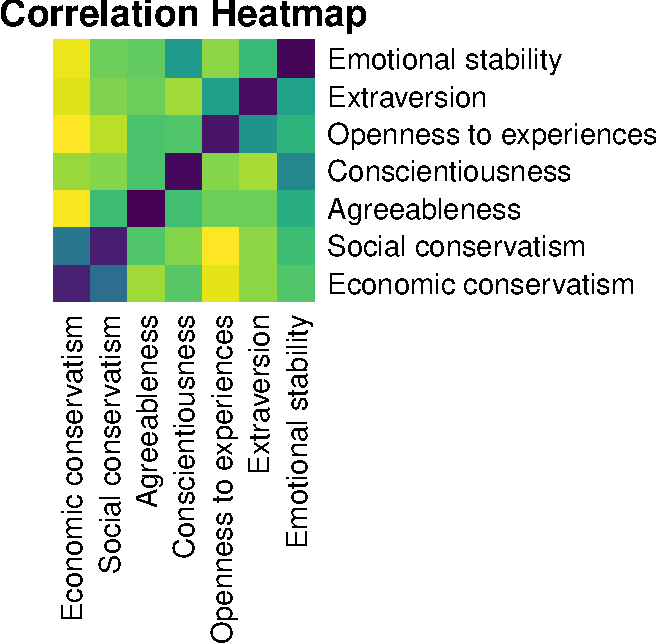
\includegraphics{manuscript_files/figure-latex/figure1-1.pdf}
\caption{\label{fig:figure1}A correlation heatmap demonstrating the
correlations between the Big Five personality traits and social and
economic conservatism.}
\end{figure}

\begin{figure}
\centering
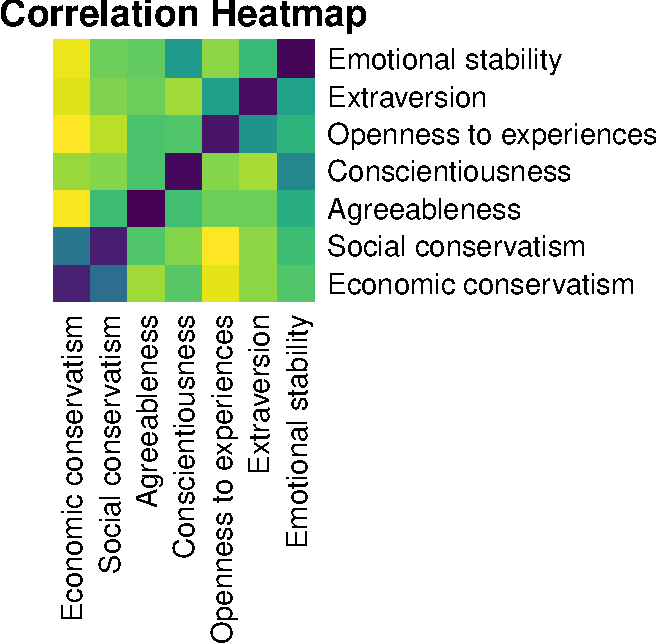
\includegraphics{manuscript_files/figure-latex/fig1-1.pdf}
\caption{\label{fig:fig1}A correlation heatmap demonstrating the
correlations between the Big Five personality traits and social and
economic conservatism.}
\end{figure}

\begin{figure}
\centering
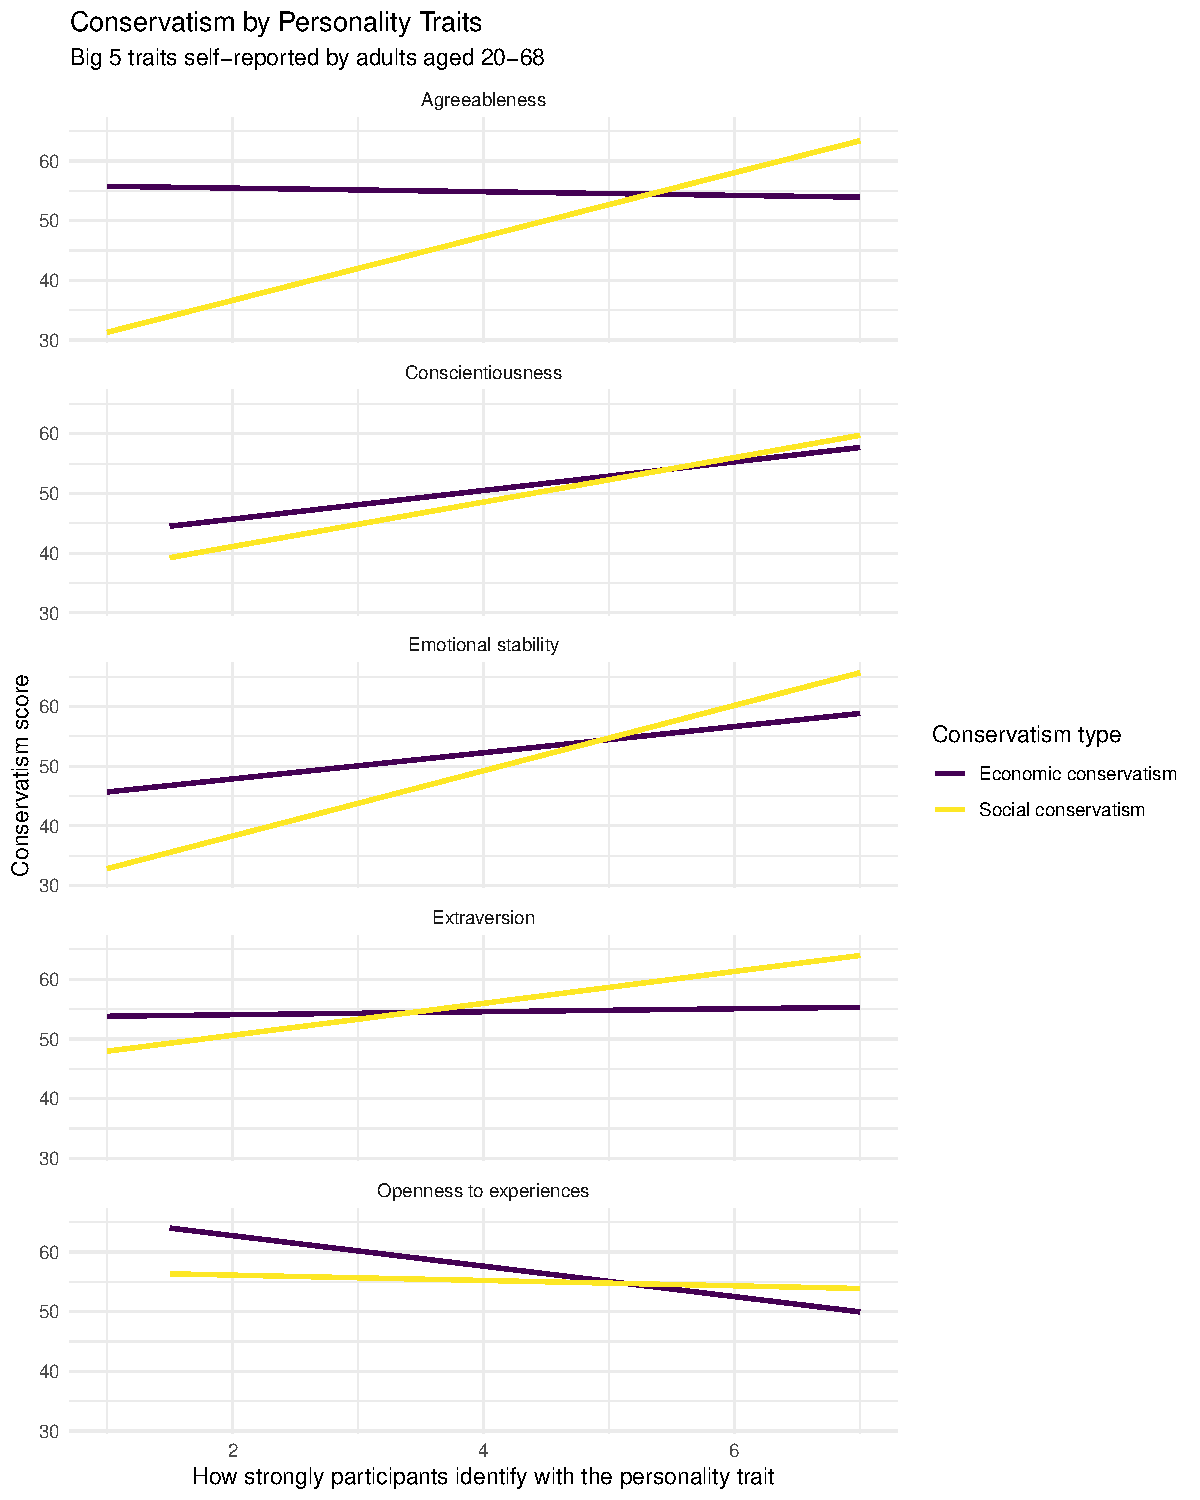
\includegraphics{manuscript_files/figure-latex/figure2-1.pdf}
\caption{\label{fig:figure2}We found a significant positive relation between
emotional stability and social conservatism, a positive relation between
agreeableness and social conservatism, and a negative relation between
openness to experiences and economic conservatism.}
\end{figure}

```

\endgroup


\end{document}
